\section{Progetto allo stato attuale}
\label{sec:progetto-allo-stato-attuale}
%
La sezione precedente ha introdotto i fondamenti teorici dell'aggregate computing, illustrando il paradigma e i framework -- \textit{ScaFi} e \textit{FCPP} -- su cui esso si basa. Questa sezione ne presenta l'applicazione concreta nel sistema \textit{Emerge}, il dimostratore realizzato dal gruppo di ricerca e punto di partenza del lavoro di tirocinio descritto in questa tesi: si illustrano dapprima l'obiettivo che ne ha guidato lo sviluppo (\cref{subsec:obbiettivo}), quindi l'architettura attraverso cui tale obiettivo è stato realizzato (\cref{subsec:archiettura-e-funzionamento}); infine si analizzano i vincoli strutturali emersi da queste scelte progettuali (\cref{subsec:vincoli}), che costituiscono il punto di partenza per l'analisi presentata nel capitolo successivo.
%
\subsection{Obiettivo}
\label{subsec:obbiettivo}
%
Il progetto di partenza, documentato in \cite{aguzzi2025demo}, nasce dall'esigenza di colmare il divario tra le fondamenta teoriche dell'aggregate computing e la sua applicazione pratica su sistemi robotici reali. Nonostante il paradigma vanti oltre un decennio di ricerca e diversi framework consolidati, le dimostrazioni su hardware fisico rimanevano limitate, rendendo difficile la transizione dal livello di maturità tecnologica TRL~3 (validazione in laboratorio) al TRL~6 (prototipo funzionante in ambiente reale) \cite{olechowski2015trl}.

L'obiettivo principale era quindi realizzare un \textbf{dimostratore pratico e open-source} per il coordinamento di squadre di robot mobili, basato sui principi dell'aggregate computing. Il dimostratore è costruito sulla libreria \textit{MacroSwarm} e sul framework \textit{ScaFi}, ed è stato concepito per essere flessibile, modulare e riutilizzabile da chiunque voglia replicare o estendere scenari analoghi.

Il progetto perseguiva tre obiettivi dimostrativi specifici. Il primo (\textbf{G1}) riguardava la formazione spaziale: mostrare come un gruppo di robot riesca a disporsi autonomamente in pattern geometrici -- come cerchio o linea -- attraverso la sola computazione aggregata, senza alcun controllo centralizzato esplicito. Il secondo (\textbf{G2}) riguardava la capacità di autoripristino (\textit{self-healing}): verificare che il sistema fosse in grado di ripristinare autonomamente la formazione desiderata in seguito a perturbazioni, come lo spostamento fisico di un robot o la rimozione temporanea di un nodo dalla squadra. Il terzo (\textbf{G3}) riguardava l'\textit{indipendenza dalla topologia}: dimostrare che la logica di coordinamento rimanesse robusta e coerente al variare del numero di robot attivi e della configurazione della rete.

Oltre agli aspetti tecnici, il progetto aveva anche una finalità divulgativa: rendere accessibili e comprensibili i concetti dell'aggregate computing a un pubblico eterogeneo, inclusi visitatori non tecnici e bambini, attraverso comportamenti visivamente intuitivi. La validazione è avvenuta in occasione della Notte Europea dei Ricercatori, dove il dimostratore è stato presentato in un contesto pubblico e interattivo.
%
\subsection{Architettura e funzionamento}
\label{subsec:archiettura-e-funzionamento}
%
Il sistema realizzato, chiamato \textit{Emerge}, è composto da quattro moduli principali -- \texttt{aruco-detector}, \texttt{neighborhood-system}, \texttt{aggregate-runtime}, \texttt{dashboard} -- che realizzano concretamente le astrazioni architetturali proposte nel modello di riferimento: \texttt{EnvironmentProvider}, \texttt{Orchestrator} ed \texttt{EnvironmentUpdate}. Ciascun modulo ha un ruolo ben definito e comunica con gli altri esclusivamente attraverso un broker \ac{MQTT} centralizzato (Mosquitto), che funge da unico bus di comunicazione dell'intero sistema. Questa scelta architetturale garantisce un disaccoppiamento naturale tra i componenti. Le connessioni tra i moduli sono illustrate in \cref{fig:connections}.

\begin{figure}
    \centering
    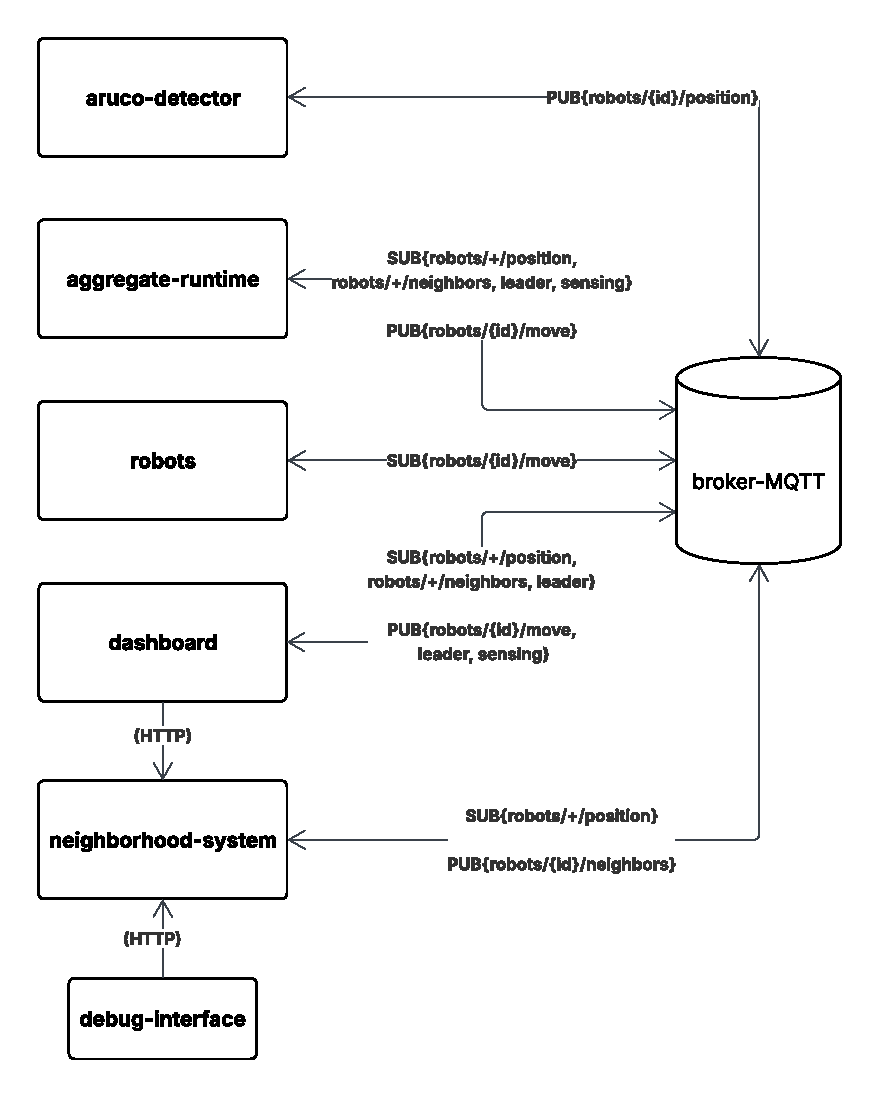
\includegraphics[width=\linewidth]{figures/background/connections.pdf}
    \caption{Connessioni tra i moduli del sistema Emerge nella versione iniziale. Le frecce indicano il flusso dei messaggi MQTT (PUB/SUB) e le chiamate HTTP verso il \texttt{neighborhood-system}.}
    \label{fig:connections}
\end{figure}

Il modulo \texttt{aruco-detector}, realizzato in Python con le librerie OpenCV e paho-mqtt, svolge il ruolo di \texttt{EnvironmentProvider}. Acquisisce in continuo il flusso video da una telecamera, individua i marker ArUco -- piccoli tag visivi applicati fisicamente su ciascun robot -- e ne ricava posizione e orientamento, pubblicando i dati aggiornati sul broker \ac{MQTT}.

Il modulo \texttt{neighborhood-system}, sviluppato anch'esso in Python tramite Flask e paho-mqtt, contribuisce alla costruzione dell'ambiente computazionale ricalcolando dinamicamente il vicinato di ciascun robot a ogni aggiornamento di posizione ricevuto dal broker. Il calcolo supporta due modalità configurabili a runtime: \texttt{full}, in cui tutti i robot attivi sono considerati vicini l'uno dell'altro, e \texttt{radius}, in cui vengono considerati vicini solo i robot entro un raggio specificato. Il vicinato aggiornato viene a sua volta pubblicato sul broker, e per consentirne la riconfigurazione senza riavviare il sistema il modulo espone alcuni endpoint HTTP, utilizzati sia dalla Dashboard sia a scopo di debug.

Il modulo \texttt{aggregate-runtime}, scritto in Scala, costituisce il nucleo computativo del sistema e svolge il ruolo di \texttt{Orchestrator} ed \texttt{EnvironmentUpdate}. È organizzato in due sottomoduli: un sottomodulo \texttt{core}, che definisce in astratto la pipeline di controllo $\texttt{EnvironmentProvider} \to \texttt{Orchestrator} \to \texttt{EnvironmentUpdate}$, parametrizzata sui tipi dominio-specifici del sistema in modo da poter essere riusata per qualsiasi squadra di robot indipendentemente da come questi sono identificati, localizzati e attuati; e un sottomodulo \texttt{demo}, che ne fornisce una realizzazione concreta per lo sciame fisico, collegando le informazioni ricevute dal broker all'esecuzione di un round ScaFi per ciascun robot e traducendone l'esito in un comando motore. I comportamenti collettivi dello sciame -- tra cui \texttt{PointTheLeader}, \texttt{VFormation} e \texttt{CircleFormation} -- sono definiti come scenari ScaFi selezionabili a runtime, senza necessità di riavviare il sistema.

Infine, il modulo \texttt{dashboard}, sviluppato in React e TypeScript, fornisce all'operatore un'interfaccia di visualizzazione e controllo in tempo reale: riceve dal broker lo stato aggiornato dello sciame e può a sua volta inviare comandi, oltre a comunicare direttamente con il \texttt{neighborhood-system} tramite HTTP per modificarne la configurazione senza passare dal broker.
%
\subsection{Vincoli}
\label{subsec:vincoli}
%
L''architettura di \textit{Emerge}, pur risultando efficace per gli obiettivi dimostrativi per cui è stata concepita, presenta alcuni vincoli strutturali che emergono direttamente dalle scelte implementative adottate.

Il vincolo più pervasivo riguarda il broker \ac{MQTT}, scelto in fase di sviluppo per la sua semplicità come unico mezzo di comunicazione dell'intero sistema. Questa decisione ha conseguenze su tutti i livelli: non solo i moduli software si parlano esclusivamente tramite Mosquitto, ma anche i robot fisici devono obbligatoriamente supportare \ac{MQTT} per poter partecipare allo sciame. Ne deriva che qualsiasi robot privo di un client \ac{MQTT} nativo -- o che utilizzi un protocollo di comunicazione diverso -- risulta di fatto incompatibile con il sistema senza interventi di adattamento. La varietà di protocolli oggi disponibili in ambito IoT rende questo un limite non trascurabile in ottica di estensibilità.

Un caso particolare è rappresentato dalla \texttt{dashboard}: poiché i browser non consentono connessioni TCP dirette verso broker \ac{MQTT} arbitrari, il modulo ricorre a \textbf{MQTT over WebSocket} (porta 9001), che incapsula i messaggi \ac{MQTT} all'interno di una connessione WebSocket. Il meccanismo funziona, ma introduce un livello di wrapping aggiuntivo che conferma come anche il componente di interfaccia sia vincolato al paradigma \ac{MQTT}, seppur con un trasporto differente.

Vale infine la pena osservare che, la localizzazione dei robot dipende interamente dalla presenza di marker ArUco fisici e dalla visibilità della telecamera: un robot non dotato di tali marker non può essere percepito dal sistema, indipendentemente da come comunica.